\documentclass[11pt,a4paper]{book}
%=============== En−Tete ===============
\usepackage[french]{babel}
\usepackage{a4wide}
%\usepackage[T1]{fontenc}
%\usepackage[cyr]{aeguill}
%\usepackage{epsfig}
%\usepackage{amsmath, amsthm}
%\usepackage{amsfonts,amssymb}
\usepackage{graphicx}
\usepackage{float}
\usepackage{url}
\bibliographystyle{plain}

\DeclareGraphicsExtensions{.png}

\title{Manuel d'utilisation Qastrocam-g2 vers. 4.4}
\author{Thx8411 \url{thx8411@users.sourceforge.net}}
%=============== Corps ===============
\begin{document}

\maketitle
\tableofcontents

\chapter{Pr\'esentation}

\chapter{Capture}

\chapter{Enregistrement}

\chapter{Autoguidage}

\chapter{Accumulation}

\chapter{Alignement}

\appendix

\chapter{Modification "latch"}

\section*{Introduction}

\paragraph*{}
Longtemps, le port parall\`ele \`a constitu\`e un outil de choix pour
interfacer un ordinateur personnel au monde ext\'erieur, notamment en
astronomie amateur. Cependant, depuis quelques années, ces ports
disparaissent de nos machines, et surtout des machines portables,
pourtant tr\`es utiles \`a l'astronome nomade.

\paragraph*{}
Le port souverain est aujourd'hui'hui l'USB, mais ce port ne permet pas l'
acc\`es direct \`a des niveaux \'electriques TTL. Les solutions envisageables
permettant donc le contr\^ole direct de ces niveaux TTL bit \`a bit sont donc de
passer par un adaptateur. Il existe des interfaces USB/parall\`ele totalement
contr\^olables pour des applications industrielles ou d'instrumentation de 
laboratoire, mais \`a des prix non n\'egligeables. Pour disposer d'une 
interface \`a un prix raisonnable, il ne reste donc que les interfaces USB/s\'erie 
ou USB/parall\`ele standards du march\'e chinois, pour quelques dollars ou euros.

\paragraph*{}
Les adaptateurs USB/s\'erie on l'avantage d'\^etre totalement contr\^olables (sur les bits)
de signalisation, du moins), mais cela ne fournit que deux bits en sortie et deux bits en
entr\'e. C'est la solution utilis\'ee par la modification longue pause s\'erie (utilisant
les lignes DTR et RTS). Il faut cependant adapter les niveaux de temsion (diverses solutions existes,
avec des jeux de r\'esistances, des transistors, des diodes zener, etc), les liaisons RS232
 fonctionnant en +/-12V. Malheureusement, cette solution ne fournie pas suffisamment de 
 sorties pour contr\^oler \`a la fois une camera longue pose et piloter l'autoguidage d'une
 monture. Pour cela, point d'autre salut que le port parall\`ele.

\paragraph*{} 
La vie \'etant sans doute trop simple, il n'est bien s\^ur pas possible de piloter directement
les niveaux de sortie d'un adaptateurs USB/parall\`ele. En effet, ces adaptateurs ne simulent pas
un port "parall\`ele", mais un port "imprimante". Cela signifie que le contr\^ole du p\'eriph\'erique
n'intervient qu'en couche haute, ou pour \^etre plus claire, qu'il est impossible de contr\^oler 
les bits de signalisation du ports, et que celui-ci n'accepte d'\'echanger des donn\'ees que
s'il est connect\'e \`a une imprimante, ou au moins quelque chose qui se comporte comme tel.

\paragraph*{}
C'est l\`a qu'intervient la modification "latch", qui consiste \`a ins\'erer le minimum d'
\'electronique permettant de simuler le comportement d'une imprimante, afin de disposer tout
de m\^eme des huit bits de donn\'ees disponibles sur le port. J'appel cette modification
"latch" car le plus gros de l'\'electronique concern\'ee est constitu\'e d'un composant TTL qui
verrouille les niveaux de sortie du port, un "latch" en anglais,un 74HC573 en l'occurence (il peut \^etre
remplac\'e par un 74HC574, voir un composant d'une autre s\'erie, type LS en fonction des
disponibilit\'es), composant tr\`es courant \`a moins de un euro.

\paragraph*{}
Le plus gros du travail provient d'ici : \url{http://www.unixgarden.com/index.php/embarque/entreessorties-simples-sur-usb}, 
avec quelques petites modifications de confort. Une LED permet de voir si le montage est sous tension, et le 
montage est auto-aliment\'e. De plus, un "reset" de l'imprimante engendre un "reset" du
verrou. La porte inverseuse du 7404 est remplac\'ee par un petit inverseur \`a transistor, moins 
encombrant qu'un CI complet.

\section*{Explications}

\paragraph*{}
Nous avons connu les "yes cards", voici venir la "yes printer". Le principe de
 base de cette modification est de faire croire que les donn\'ees sont toujours lues
 correctement, que l'imprimante et toujours disponible, et que tout se passe toujours bien.
  Pour cela, une partie des
 signaux est directement renvoy\'ee \`a l'ordinateur, comme accus\'e r\'eception, et
 une autre for\'ee au niveau bas, \`a la masse. Pendant ce temps, le signal de 
 synchronisation du PC sera utilis\'e pour stocker les donn\'ees dans le verrou.
 
 \paragraph*{}
 Un bon dessin \'etant bien mieux qu'un long discours, le sch\'ema est visible sur la figure~\ref{latch1}.
 
 \begin{figure}
 \center
 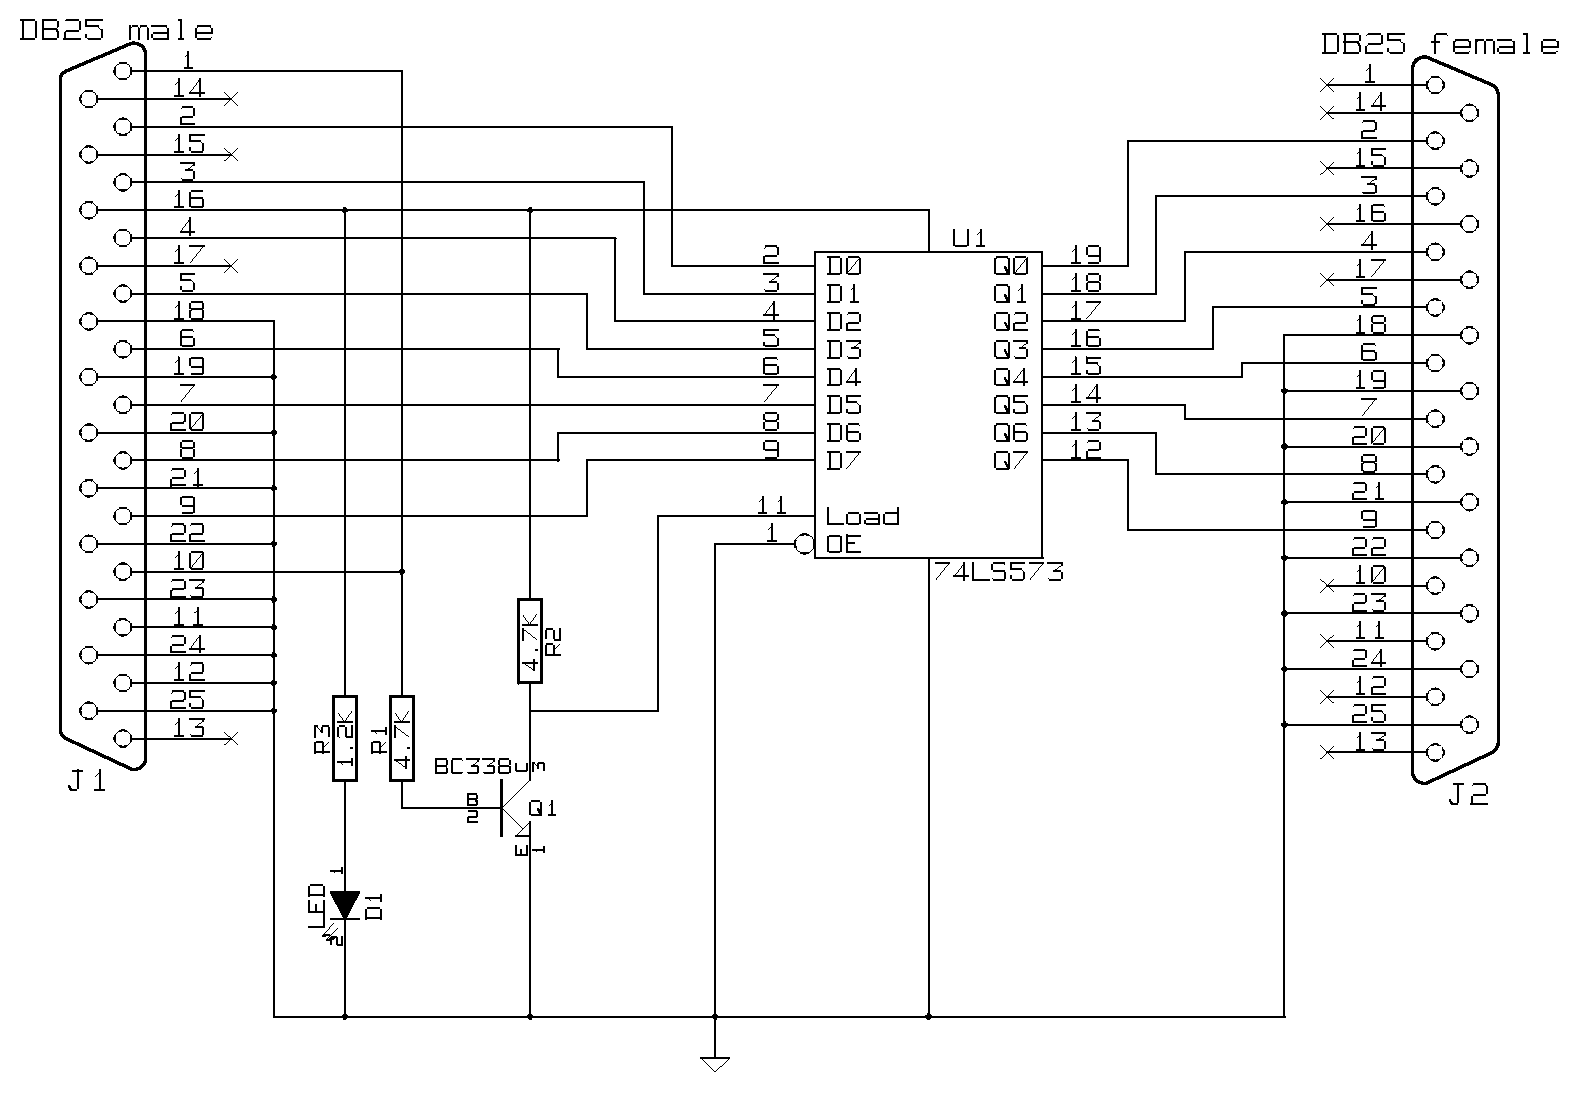
\includegraphics[scale=1.1]{./medias/latch1.png}
 \caption{sch\'ema}
 \label{latch1}
 \end{figure}
 
\paragraph*{}
Le PC se trouve cot\'e J1, et l\'el\'ement ext\'erieur \`a contr\^oler cot\'e J2. Les pins \`a
la masse des deux connecteurs sont mis \`a la masse du montage, et les pins de donn\'ees 
respectivement connect\'ees \`a l'entr\'e et \`a la sortie du verrou. Sur J2, aucun des bits
de signalisation ne sont report\'es. Normal, nous n'y avons de toute fa\,con pas acc\`es.
C'est au niveau des bits de signalisation de J1 que les choses se jouent.

\paragraph*{}
Le signal {\tt INIT} (16) nous serre d'alimentation pour le montage. Il est en effet maintenu \`a
{\tt HIGH} par la pc, sauf lors de l'envoi d'un {\tt RESET} \`a l'imprimante, ce qui nous permet 
\'egalement de faire un {\tt RESET} du verrou. Ce signal alimente donc le verrou, un petit t\'emoin
\`a LED ainsi qu'un inverseur \`a transistor dont nous reparlerons plus loin. Il est \`a noter
que les signaux d'un port parall\`ele sont fait pour piloter des portes logiques, il est donc 
important d'en tirer le moins de courant possible. La LED sera donc de pr\'ef\'erence une LED
faible courant, avec une r\'esistance de limitation adapt\'ee. De toute mani\`ere, en application
astronomique, il est conseill\'e d'avoir le moins de lumi\`ere parasite possible, la LED et sa r\'esistance 
peuvent donc \^etre omises au besoin. De m\^eme pour les donn\'ees en sortie, il est imp\'eratif que 
celles-ci soient reli\'ees \` des entr\'es haute imp\'edance.

\paragraph*{}
 Notre imprimante n'est jamais occup\'ee et a toujours du papier, les entr\'es {\tt BUSY} (11) et
 {\tt PAPEROUT} (12) sont donc reli\'ees \` la masse. L'entr\'ee {\tt /ACK} (10) est directement reli\'ee
 \`a la sortie {\tt STROBE} (1). Notre imprimante accuse automatiquement r\'eception de tout ce
 qu'elle re\,coit. {\tt STROBE}, via notre inverseur,pilote \'egalement le chargement de notre
 verrou. Sur notre verrou, les donn\'ees doivent \^etre en permanence disponibles en sortie,
 {\tt /OE} est donc mise \`a la masse.
 
 \paragraph*{}
 Les autres signaux, {\tt SELECT} (13), {\tt AUTOFEED} (14), {\tt ERROR} (15) et 
 {\tt SELECTIN} (17) n'ont pas besoin d'\^etre g\'er\'es, ils sont donc simplement ignor\'es. 
 
\section*{R\'ealisation}

\paragraph*{}
La r\'ealisation ne devrait pas poser de probl\`emes. Pour tous ceux qui n'ont pas les moyens
mat\'eriels de graver des circuits imprim\'es, le montage sur une plaque de test est assez
simple, vu le faible nombre de composants. Pour les autres, voici le typon (figure~\ref{latch2}) 
ainsi que la s\'erigraphie (figure~\ref{latch3}) du montage. Les pistes sont volontairement
tr\`es larges pour permettre une r\'ealisation avec les moyens du bord facile.

\paragraph*{}
Si tous se passe bien, vous devriez obtenir un circuit semblable \`a la figure~\ref{latch3}.

\begin{figure}
 \center
 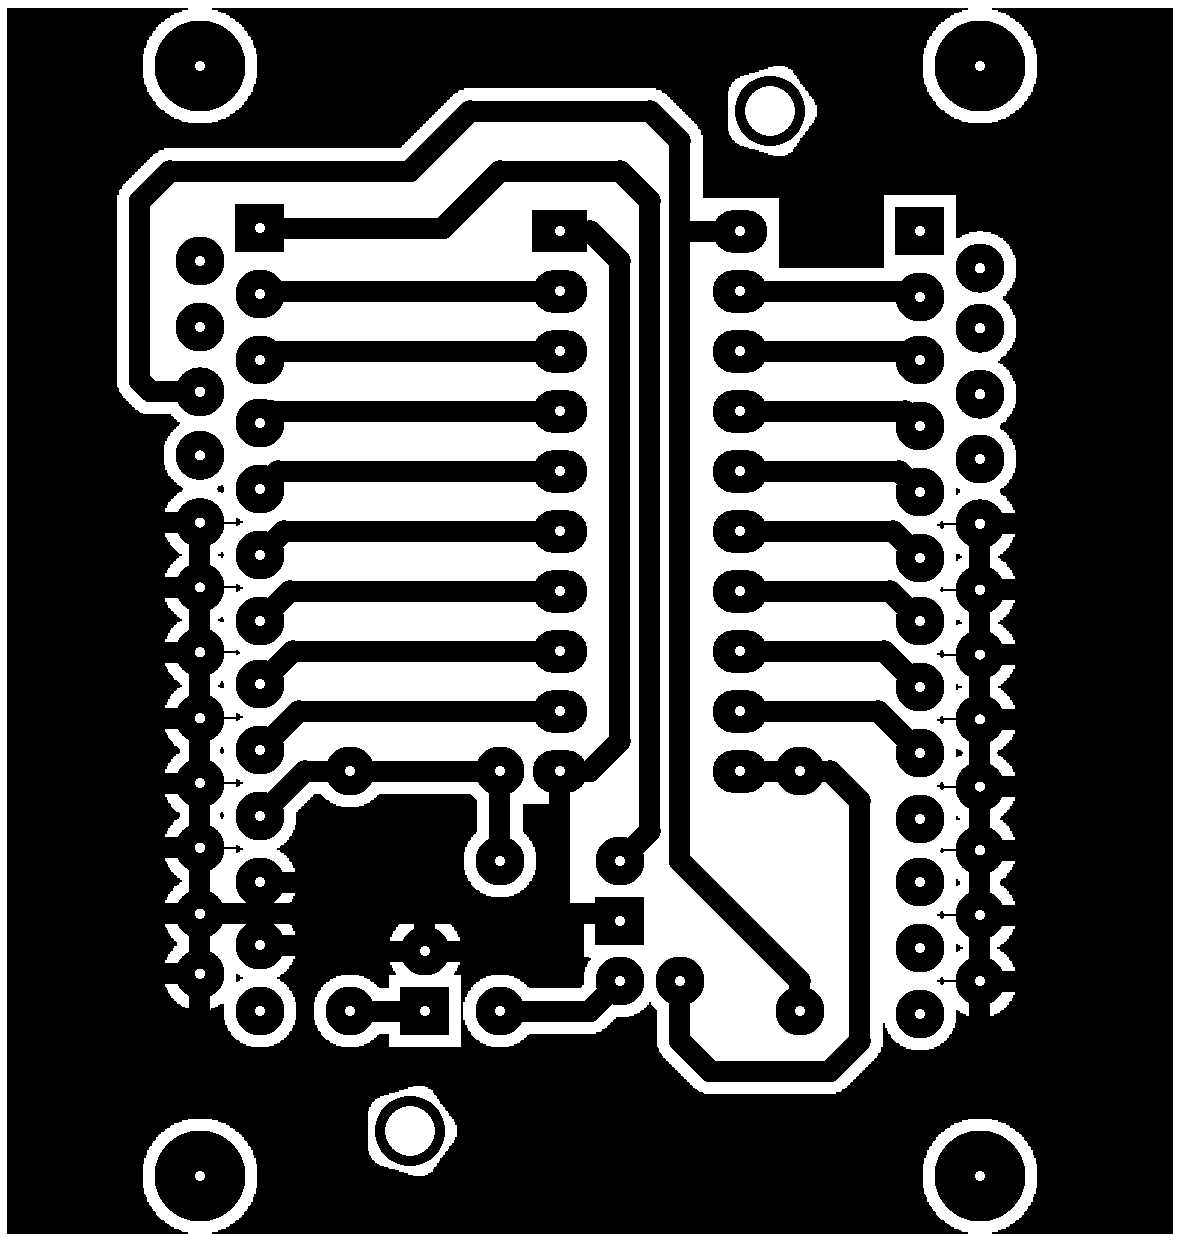
\includegraphics[width=5cm]{./medias/latch2.png}
 \caption{typon}
 \label{latch2}
 \end{figure}
 
 \begin{figure}
 \center
 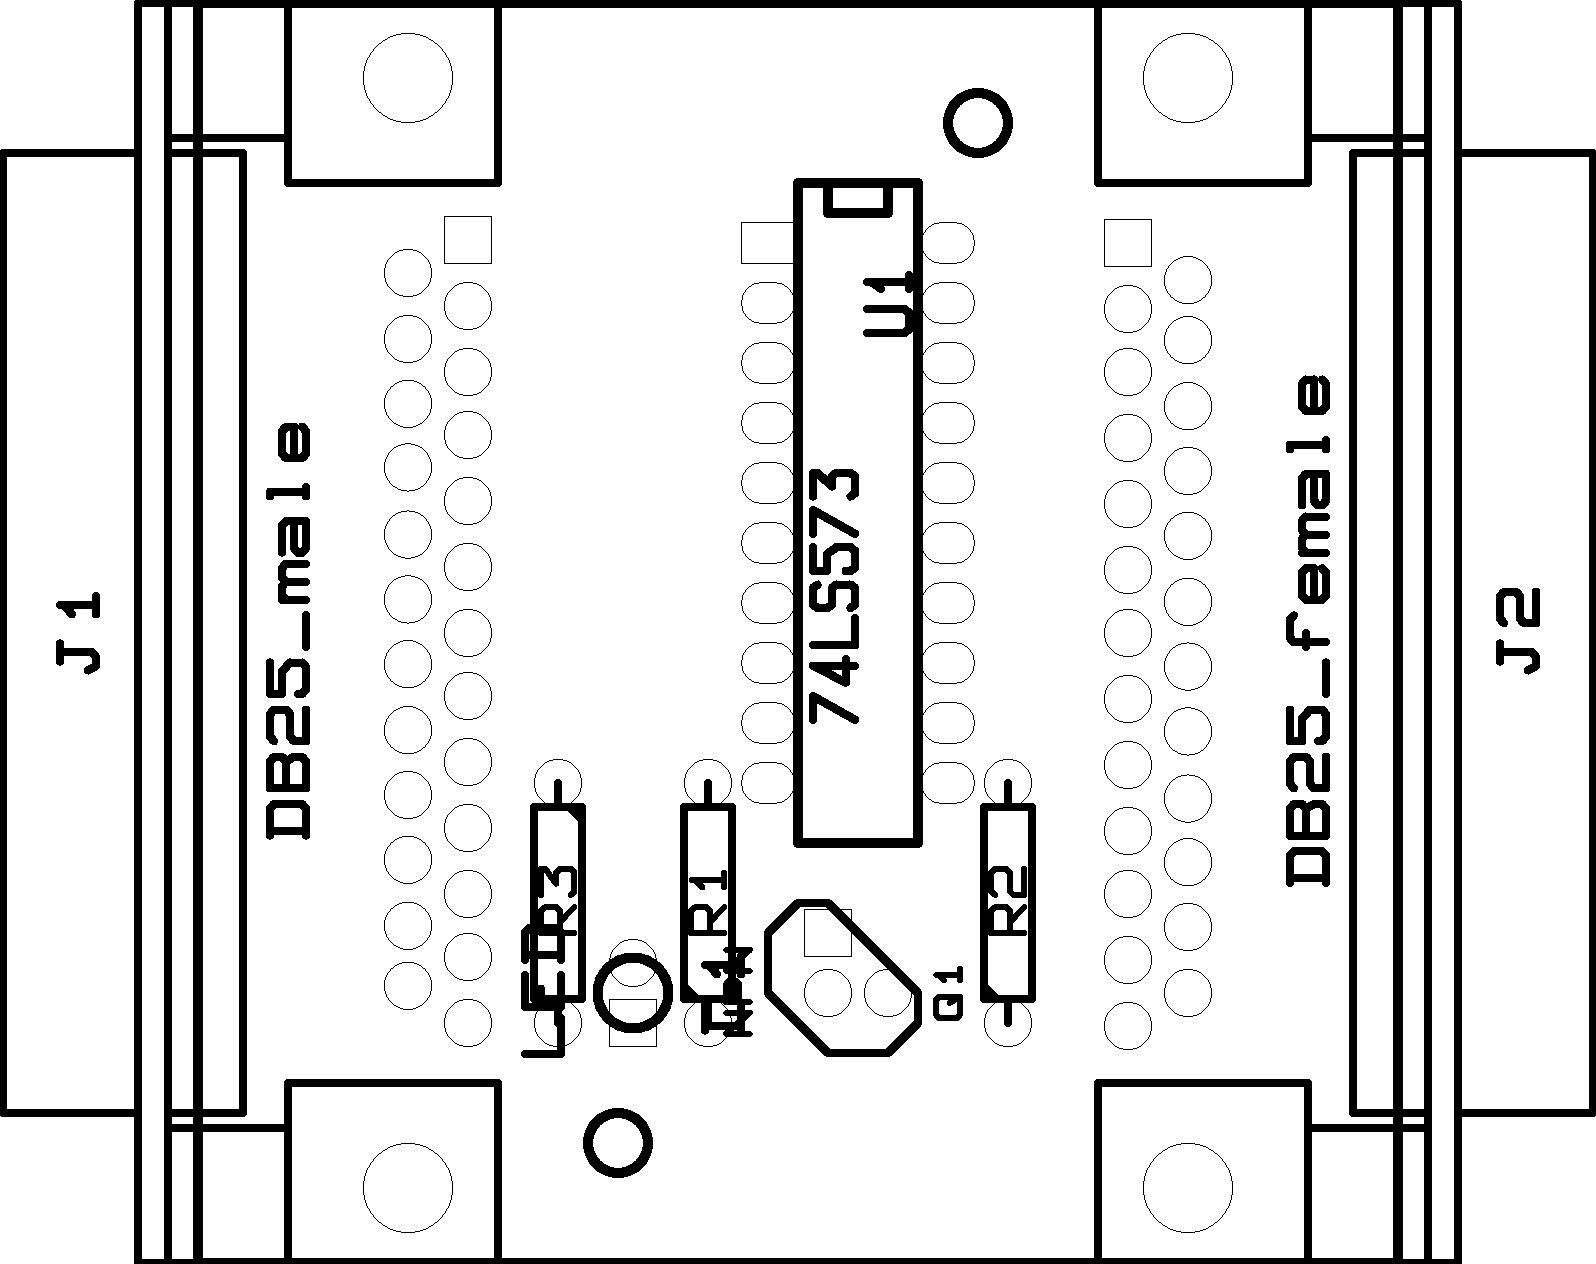
\includegraphics[height=52mm]{./medias/latch3.png}
 \caption{s\'erigraphie}
 \label{latch3}
 \end{figure}
 
 \begin{figure}
 \center
 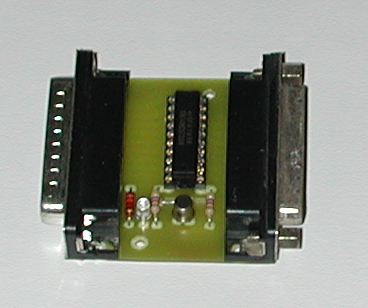
\includegraphics[scale=1.1]{./medias/latch4.png}
 \caption{montage}
 \label{latch4}
 \end{figure}
 
 \paragraph*{}
 Je vous recommande de placer tout ceci dans une petite boite, pour le prot\'eger de l'humidit\'e
 de vos sorties nocturnes...

\section*{Mise en oeuvre}

\paragraph*{}
Une fois ce petit montage branch\'e deri\`ere votre adaptateur USB/parall\`ele, il vous est
possible d'envoyer un octet directement en ouvrant le p\'eriph\'erique {\\tt /dev/lp?} 
correspondant et en y \'ecrivant un {\tt unsigned char} (ou l\'equivalent dans un autre langage).
L'appel \`a la fonction {\tt ioctl} {\tt LPRESET} vous permet de r\'einitialiser le verrou. Je vous
recommande simplement d'ins\'erer un d\'elai d'une micro-seconde entre deux \'ecritures sur votre
port parall\`ele, vous respectez ainsi le "timing" standard de l'IEEE 1284.

\paragraph*{}
Je rappel qu'il est tr\`es important de tirer le moins de courant possible de ce montage, et que
 l\'equipement dispos\'e en aval devra imp\'erativement disposer d'entr\'ees haute imp\'edance !

\listoffigures

\end{document}
